\documentclass[amsmath,amssymb,notitlepage,12pt]{revtex4-1}
\usepackage{graphicx}
\usepackage{bm}% bold math
\usepackage{multirow}
\usepackage{booktabs}
\usepackage{verbatim}
\usepackage{hyperref}
\hypersetup{pdftex,colorlinks=true,allcolors=blue}
\usepackage{hypcap}
%\usepackage[0.1]{vrsion}

\begin{document}
\hspace*{11.5cm}CLAS-NOTE 2013-009


\title{RTPC Gain Calibration for EG6}
\author{N. Baltzell}
\affiliation{Argonne National Laboratory}
\date{\today}
\begin{abstract}
The Radial Time Projection Chamber of EG6 is gain-calibrated with $^4$He nuclei elastically scattered by 1.2 GeV electrons.
\end{abstract}
\maketitle
\tableofcontents

\section{Introduction}
The Radial Time Projection Chamber (RTPC) detects low energy nuclear recoils from EG6's $^4$He target well below the threshold of CLAS.  The timing of the RTPC hits allows measurement of $\vec{p}/q$ via the drift path calibration and a helix fit.  Then a measurement of energy deposition and gain calibration gives $\frac{dE}{dx}$ and particle identification.

To calibrate the gains of the 3200 RTPC channels, a selection of cleanly measured tracks of known particle type is desired.  For this, first good drift paths calibrations are required~\cite{driftpaths}.  Then elastic scattering events, with the electron measured in CLAS and the $^4$He in the RTPC, are used to adjust the gains to match the expected $\frac{dE}{dx}$.

\section{Rate of Energy Loss}
The ratio of the measured and expected values of $\frac{dE}{dx}$ is the basis of the gain calibration.  By scaling the ADC of each hit by its GEM pad's gain factor, the measured $\frac{dE}{dx}$ can be calibrated to match, on average, the expected distribution from the ``Bethe'' equation. % Only elastically scattered $^4$He in the RTPC from EG6's low beam energy calibration data are used.
%Then the gains are adjusted  such that the measured $\frac{dE}{dx}$ vs $p$ falls along the ``Bethe'' equation for moderately relativistic $^4$He nuclei.

%to be used for particle identifaction.
%for particle identification via elastic $^4$He tracks.
%gains of the RTPC's 3200 channels for particle identification.

%Timing information from the Radial Time Projection Chamber (RTPC) results in measurement of $\vec{p}/q$, and combining that with energy information allows measurement of $\frac{dE}{dx}$.
%with is document describes the method currently used to calibrate the gains of the RTPC based upon elastic $^4$He elastic scattering.

%Only elastically scattered $^4$He in the RTPC from EG6's low beam energy calibration data are used.
%to ensure a cleanly measured sample of known species.  This relies on good calibration of the RTPC drift paths \cite{driftpaths} and electron detection in CLAS.

%\section{Rate of Energy Loss}
%The ratio of the measured and expected values of $\frac{dE}{dx}$ is the basis of the gain calibration.  By scaling the measured ADC of each hit by its GEM pad's gain factor, the measured $\frac{dE}{dx}$ can be calibrated to match, on average, the distribution from the ``Bethe'' equation.
\subsection{Expected Energy Loss}
The expected average rate of energy loss due to ionization is described by the ``Bethe'' equation for heavy charged particles \cite{pdg}:
\begin{equation}
    -\left\langle\frac{dE}{dx}\right\rangle = \rho Kz^2\frac{Z}{A}\frac{1}{\beta^2}\left[\frac{1}{2}\ln{\frac{2m_ec^2\beta^2\gamma^2T_{max}}{I^2}-\beta^2-\frac{\delta(\beta\gamma)}{2}}\right]
\label{eq:bb}
\end{equation}
where $T_{max} = \frac{2m_ec^2\beta^2\gamma^2}{1+2\gamma m_e/M+(m_e/M)^2}$ and $K=0.307075$ MeV/g$\cdot$cm$^2$.  The variables $z$, $M$, and $\beta$ are the particle's charge, mass and speed, while $Z$, $A$, and $I$ are the ionization medium's effective atomic charge, number, and ionization energy, and $\rho$ its mass density.  The $\delta$ term is neglected and not important at our energies.

The properties of the EG6 drift gas are shown in Table \ref{tab:gasprop}.  The ionizaion energy affects the shape of the $\frac{dE}{dx}$ distribution, while the rest of the parameters serve only as absolute normalization factors.  Applying these parameters to Eq. \ref{eq:bb} results in the expected dependence of energy deposition on momentum for the 5 possible recoil particles in Fig. \ref{fig:bb}.

With the RTPC timing and drift paths calibration, the measured momentum $p/q$ can be used as input to Eq. \ref{eq:bb} to determine the expected $\frac{dE}{dx}$ for each track if the particle type is known.
\begin{table}[tbp]
    \caption{\label{tab:gasprop}Properties of EG6 RTPC Drift Gas}
    \begin{tabular}{p{4cm}r}
    \toprule[1.5pt]
    \multicolumn{2}{c}{Ne:DME 80:20} \\ \cmidrule[0.5pt]{1-2}
    Pressure & 1 atm \\
    Density & 1.03 mg/cm$^3$\\
    $Z_{eff}$ & 66 \\
    $A_{eff}$ & 126.79 \\
    $I_{eff}$ & 99.79 eV\\
    \bottomrule[1.5pt]
\end{tabular}
\end{table}
\begin{figure}[tbp]\centering
    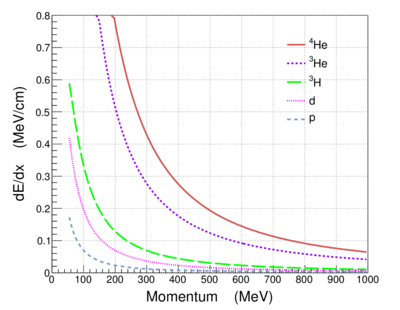
\includegraphics[width=10cm]{bb_small.png}
    \caption{The expected mean energy loss in EG6 RTPC's drift gas.\label{fig:bb}}
\end{figure}

\subsection{Measured Energy Loss}\label{sec:measureddedx}
The measured energy loss for a track is calculated by summing over the charges measured in each hit in the track and dividing by the total path length:
\begin{equation}
    \left\langle\frac{dE}{dx}\right\rangle = \sum_{i} \frac{\textrm{ADC}_{i}}{G_{i}}\ /\ L
    \label{eq:dedxmeas}
\end{equation}
There are 3200 gain scaling factors $G_i$, one for each readout pad, and determining their values is the goal of the gain calibration.
The path length $L$ of the track in the drift region is calculated from the result of a helix fit between the point of the first hit and the last hit measured in the RTPC. 

%\subsubsection{Bad Path Length}\label{sec:badpad}
However, the recoil's trajectory through the drift region can intersect malfunctioning readout pads.  Those segments of the path length should be discarded from the calculation of $L$ in Eq. \ref{eq:dedxmeas}. This is achieved by first identifying the bad pads, and then using the reverse of the drift paths calibration, $(r,z,\phi)\rightarrow($pad\#$)$, to identify the portions of the path length that would have deposited energy on those pads.

%The relevant distance along the helix starts at the position of the first measured charge and ends at the last.
By stepping along the path length in between the first and last hits in sufficiently small increments and calculating the expected pad hit, the fraction associated with bad pads can be estimated.
This fraction is stored in the {\it RTPC} bank's variable {\it bad}.  The effect is most significant near regions of consecutive bad pads, as shown in Fig. \ref{fig:badpad}.
The measured $\frac{dE}{dx}$ is recalculated using the corrected path length and stored in the {\it RTPC} bank's {\it dedx2}, and this is the value used for the calibrations.
%The corrected path length is not stored directly, but can be recalculated from $\frac{\texttt{rtpc\_dedx}}{\texttt{rtpc\_dedx2}}\times\texttt{vtl[rtpc\_gcpb]}$ 
%or $\frac{\texttt{vtl[rtpc\_gcpb]}}{\texttt{rtpc\_bad}}$
\begin{figure}[htbp]\centering
    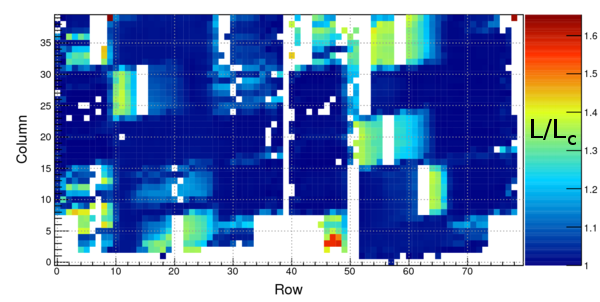
\includegraphics[width=11cm]{DedxBPCratio_small2.png}
    \caption{The ratio of the path length calculated without and with a correction for bad pads shown over the surface of the GEM.  Only elastic $^4$He are shown.\label{fig:badpad}}
\end{figure}

\section{Analysis}
\subsection{Elastic Event Selection}
Events with exactly one electron detected in CLAS are selected.  Electron identification requires a track in the drift chambers with curvature corresponding to negative charge and energy deposition in the EC consistent with that expected for electrons ($E_{\textrm{inner}}>80MeV$ and $0.2<E_{\textrm{tot}}/p<0.4$ in {\it epass1v11} data).  After this, at 1.206 GeV beam energy, the electron sample is already sufficiently clean without using CC information.

Next, good tracks reconstructed in the RTPC are selected.  To do so, cuts are placed on the helix fit parameters in Table \ref{tab:rtpccuts1}, where $sdist$ ($edist$) is the distance along the helix between the first (last) detected hit to the cathode (GEM).  The $z$-vertex cut is asymmetric to remove the tracks that would have passed through the upstream target holder.
\begin{table}[thpb]
    \caption{\label{tab:rtpccuts1}RTPC Track Quality Cuts}
    \begin{tabular}{c}
    \toprule[1.5pt]
    -84 mm $<$ $z$-vertex $<$ +100 mm \\
    -5 mm $<$ edist $<$ +5 mm \\
    -2 mm  $<$ sdist $<$ +5 mm \\
    0.3   $<$ $\chi^2$ $<$  3 \\
    $N_{\textrm{pads}} > 3 $\\
    $r_0>0$ \\
    \bottomrule[1.5pt]
\end{tabular}
\end{table}
%A $z$-vertex match is required between the RTPC track and the CLAS electron; the peak is shown in Fig. \ref{fig:dz}.
%\begin{figure}[htbp]\centering
%    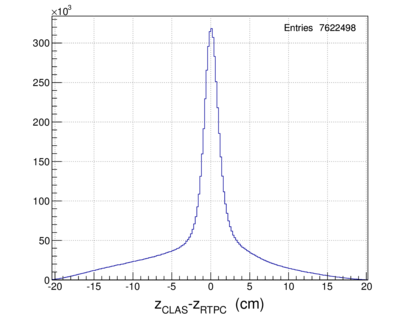
\includegraphics[width=8cm]{dz_small.png}
%    \caption{The $z$-vertex difference between electrons and all RTPC tracks.\label{fig:dz}}
%\end{figure}

Based upon momentum conservation for elastic scattering, the expecetd $^4$He recoil angles calculated from the electron are compared to that measured by the RTPC, and 3-$\sigma$ cuts are placed around the peaks in Fig. \ref{fig:elastics}. 
The resulting elastic peak in the right panel of Fig. \ref{fig:elasticsW} (red histogram) demonstrates the clean selection of $^4$He tracks in the RTPC, and these $\sim$500K tracks are used for gain calibration.% in the next section.
%An additional $p/\theta$ cut on the elastic electron peak is also used for an extra clean sample.
\begin{figure}[htbp]\centering
%    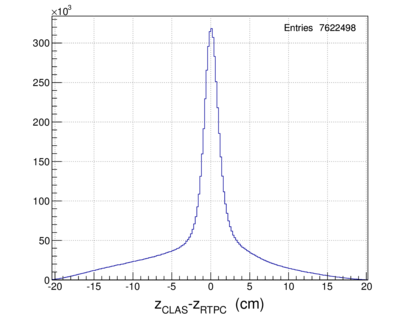
\includegraphics[width=5.4cm]{dz_small.png}
%    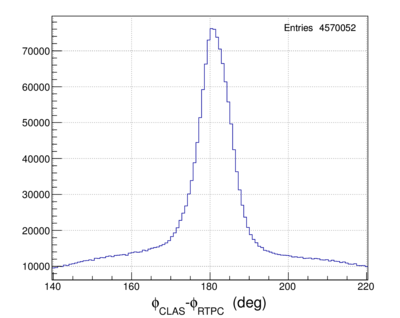
\includegraphics[width=5.4cm]{dphi_small.png}
%    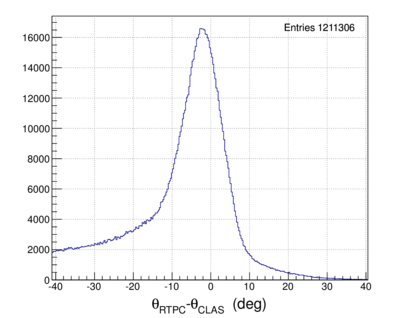
\includegraphics[width=5.4cm]{dthe_small.png}
%    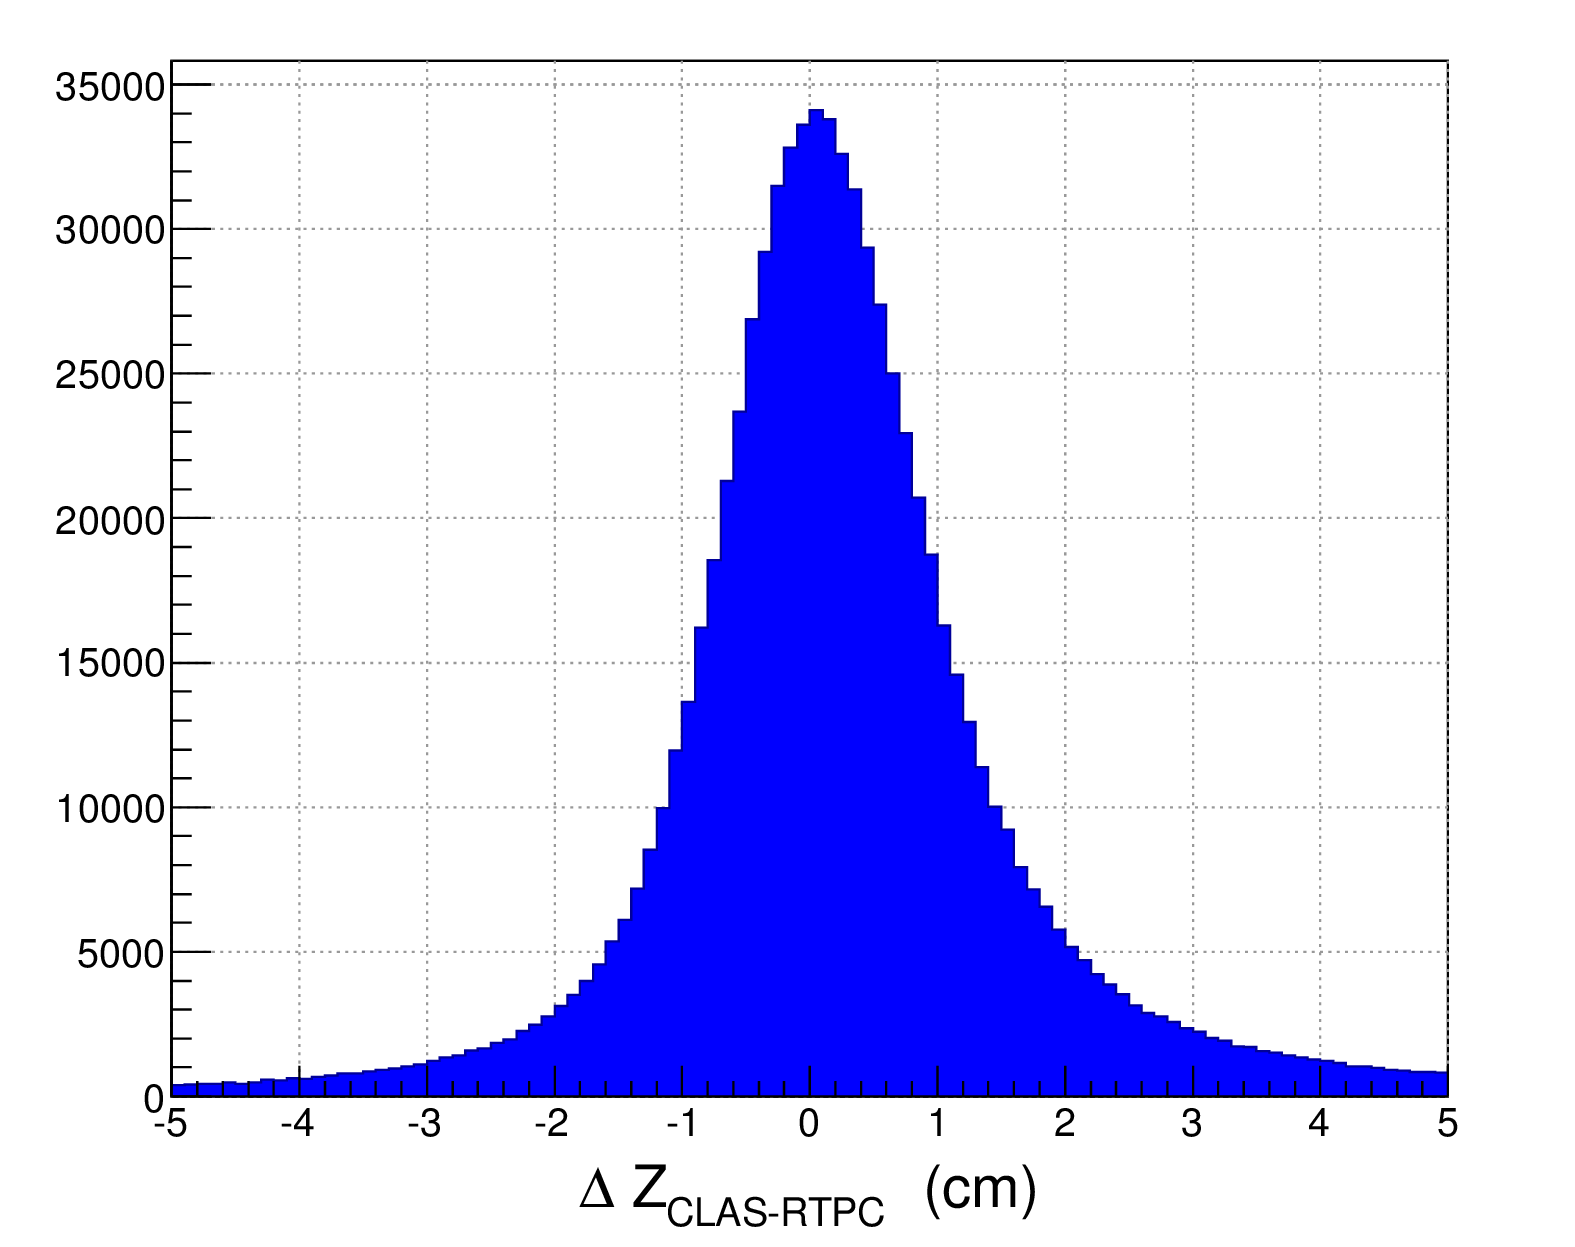
\includegraphics[width=5.4cm]{dz_othercuts.png}
%    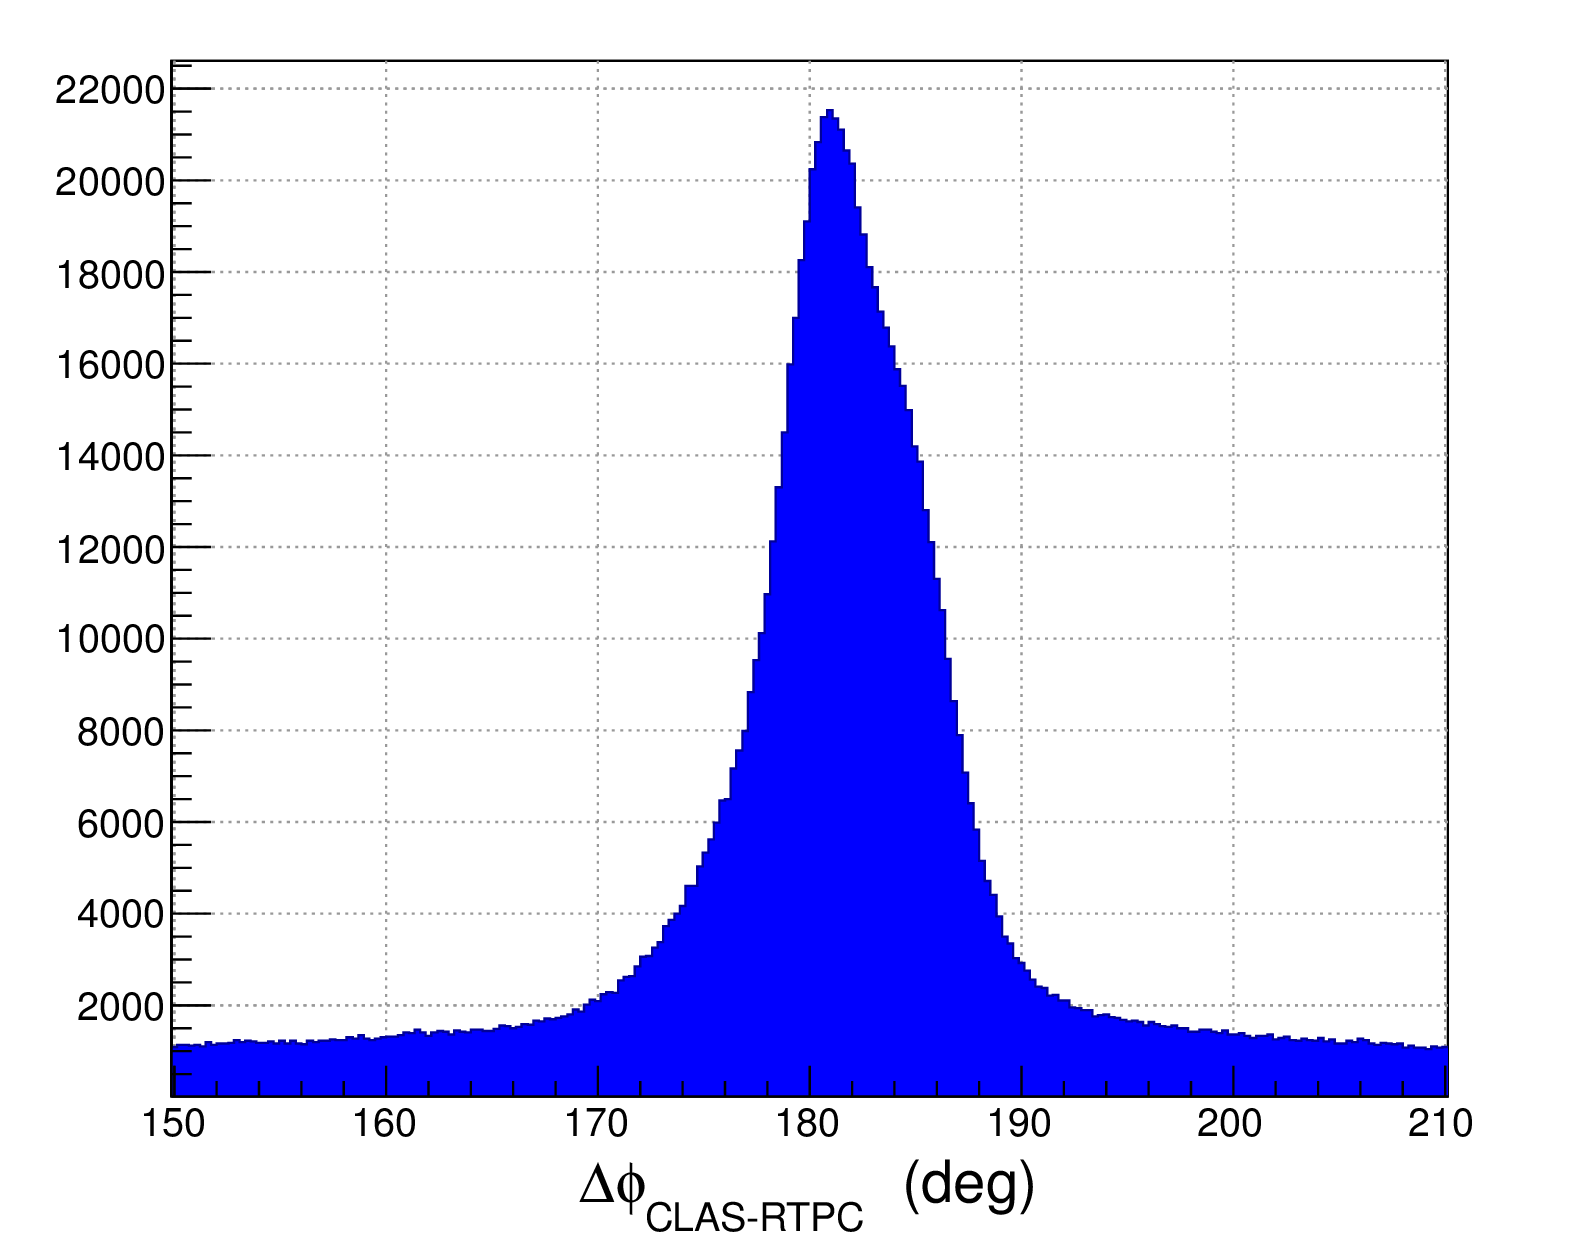
\includegraphics[width=5.4cm]{dphi_othercuts.png}
%    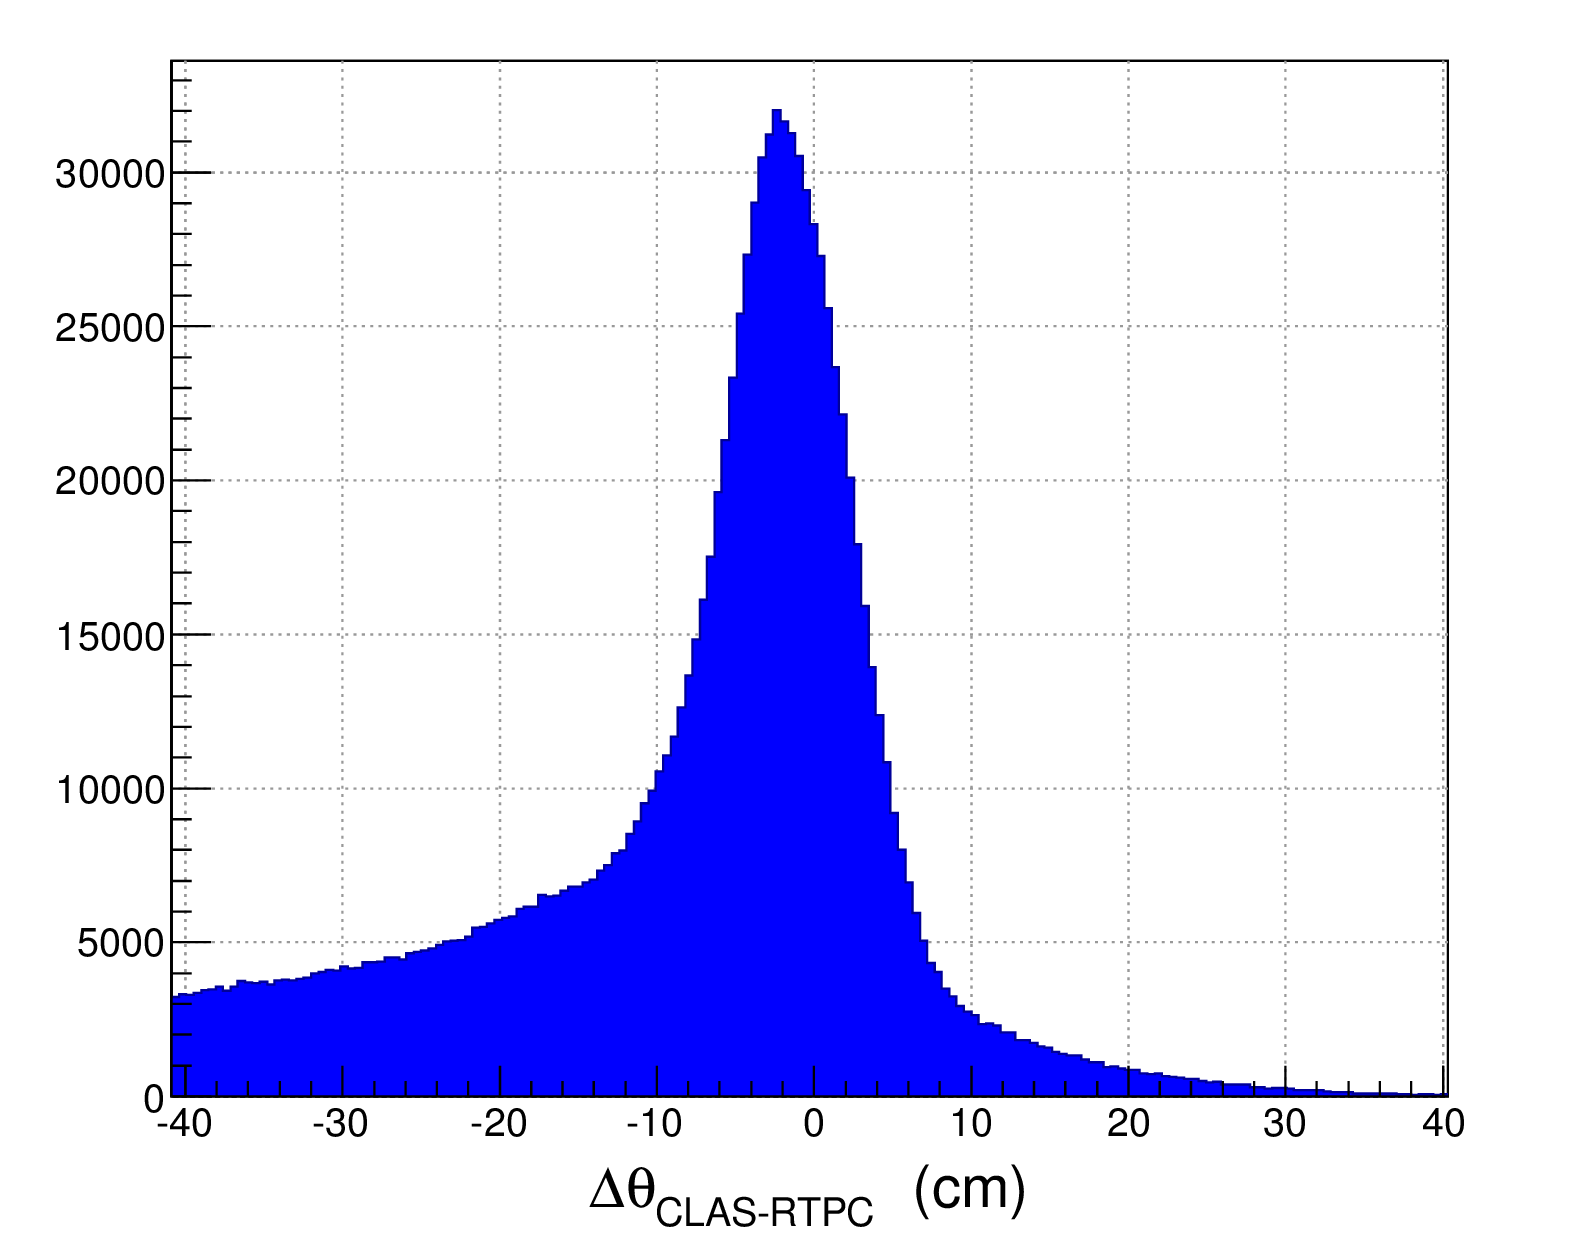
\includegraphics[width=5.4cm]{dthe_othercuts.png}
    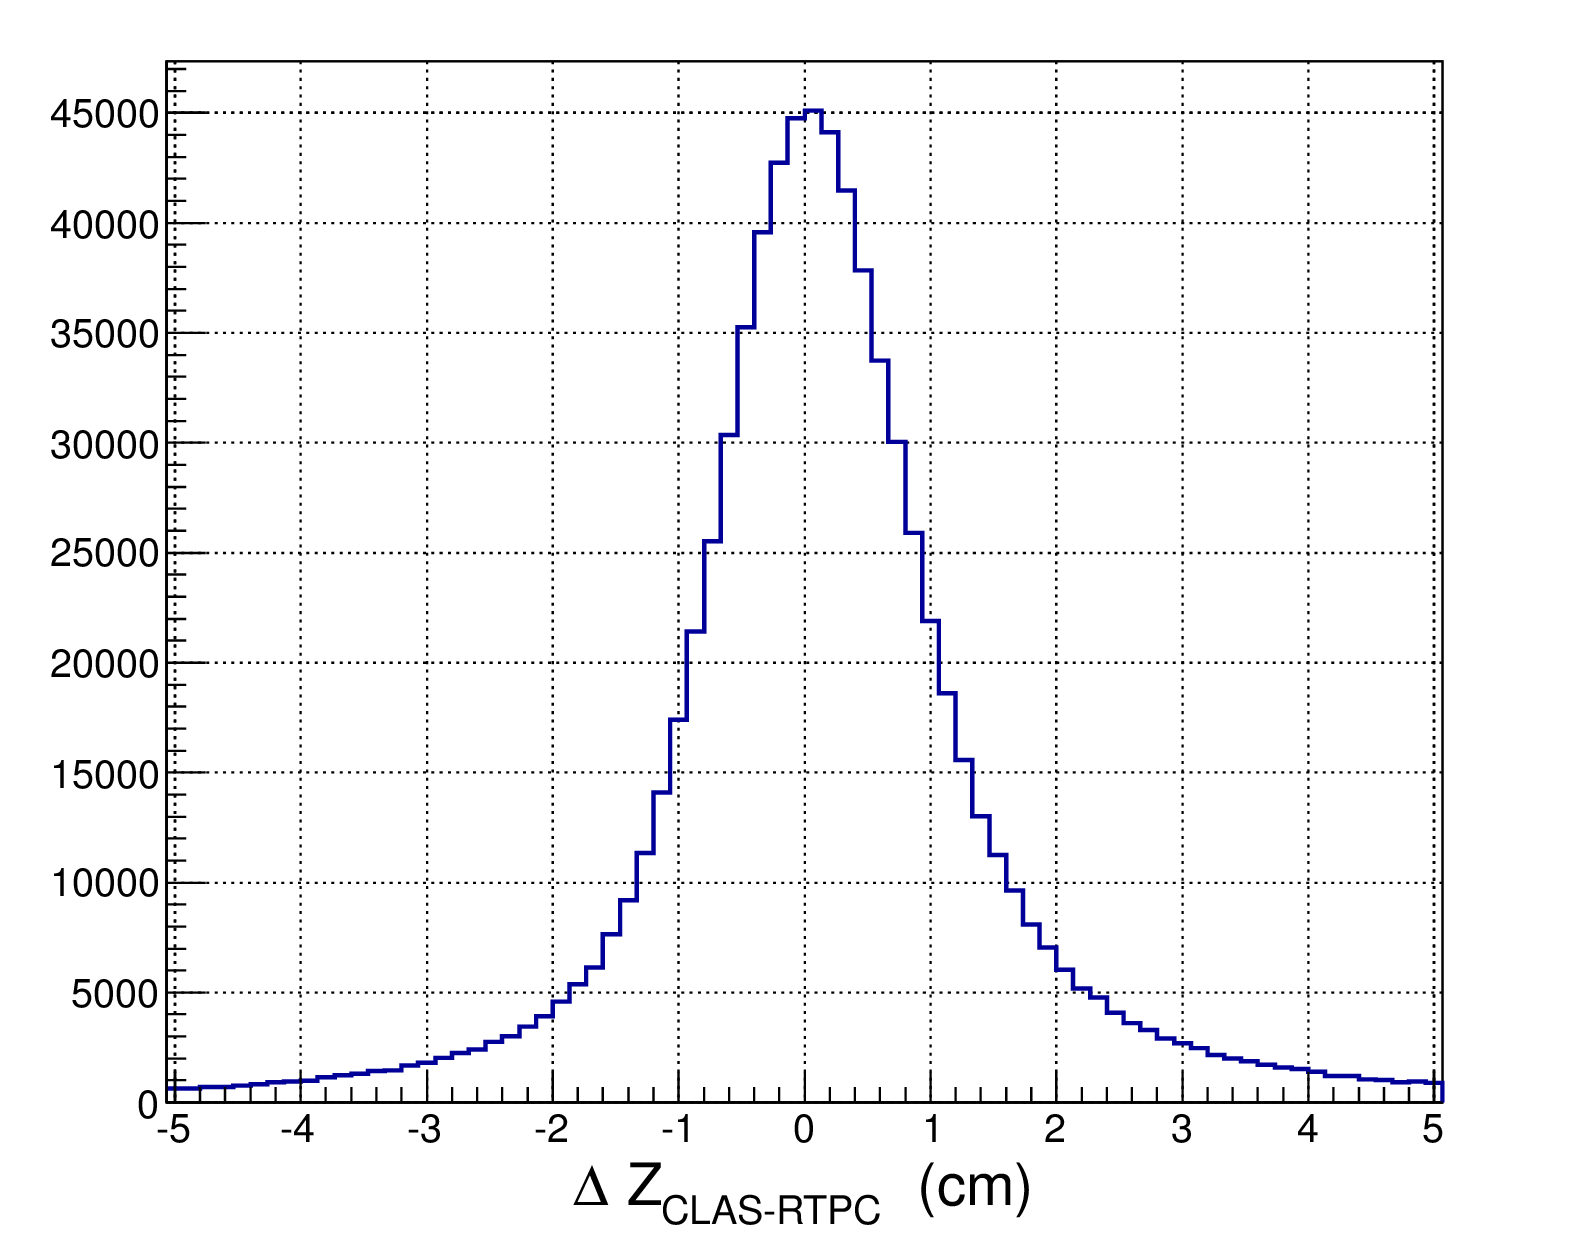
\includegraphics[width=5.4cm]{dzQ.png}
    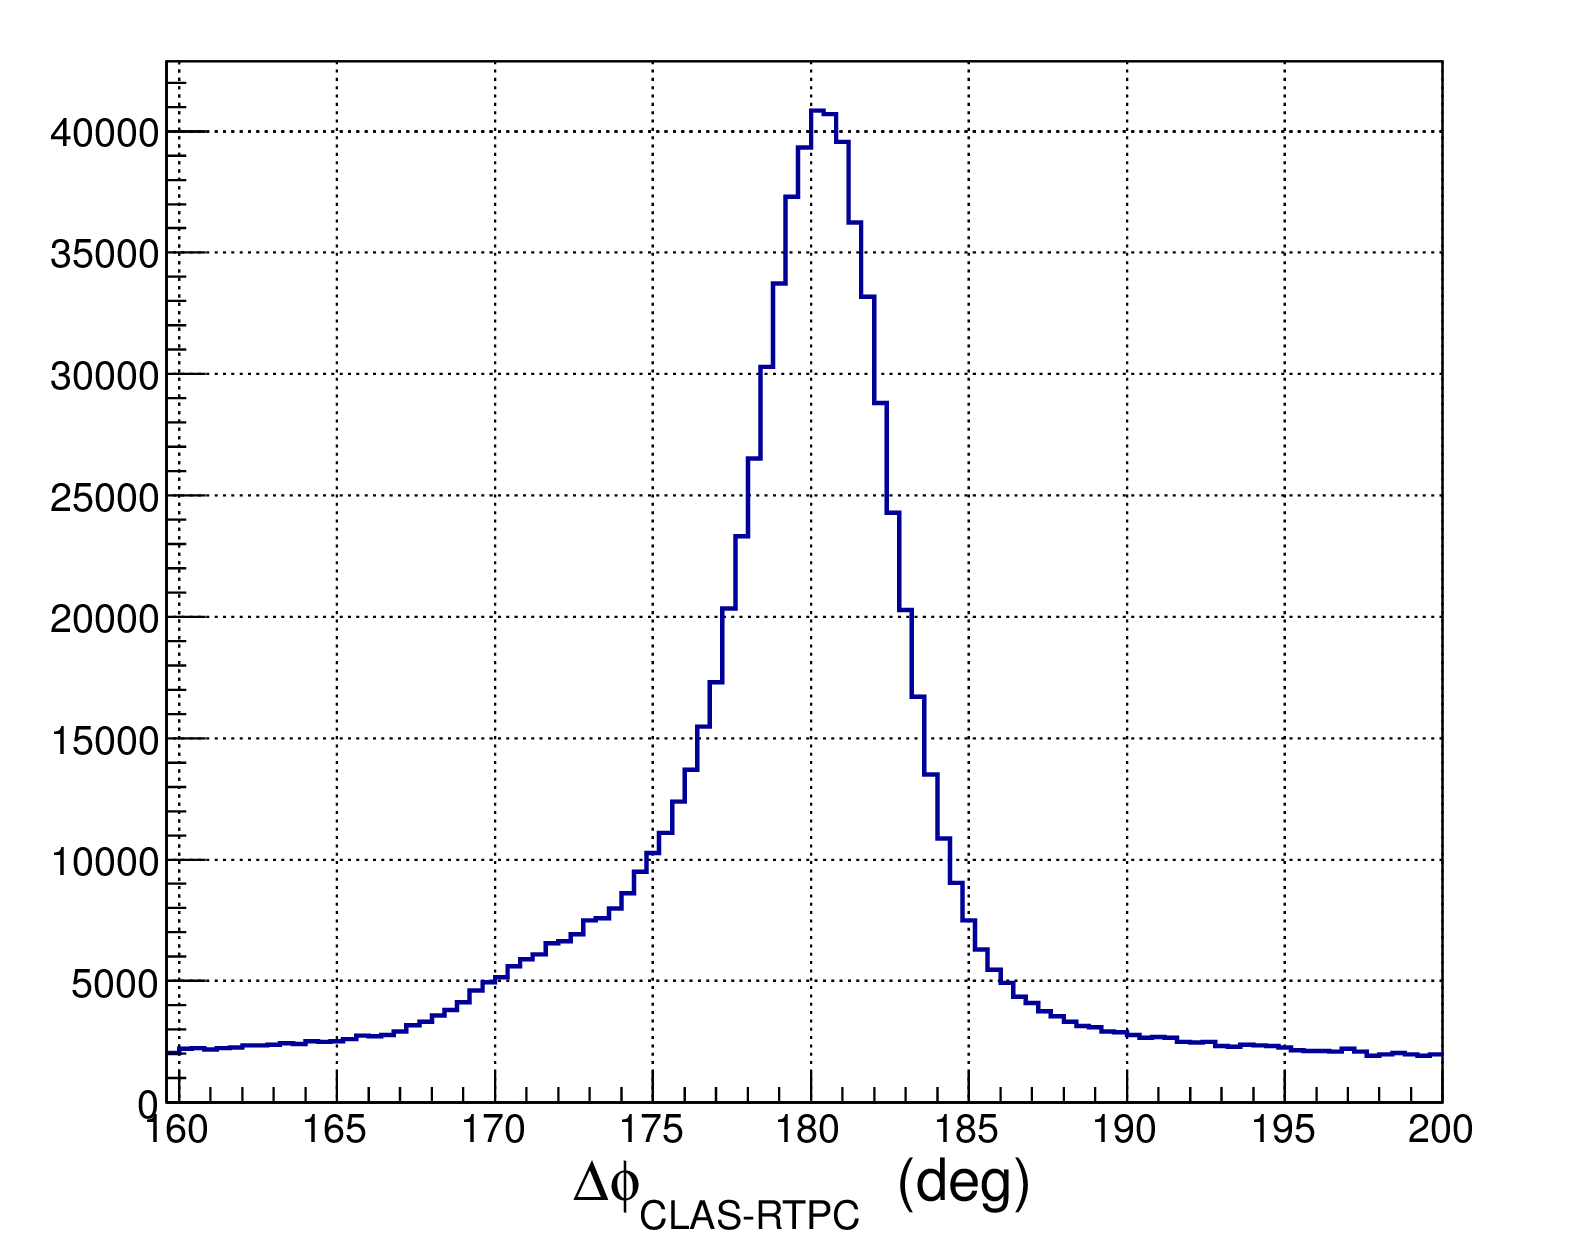
\includegraphics[width=5.4cm]{dphiQ.png}
    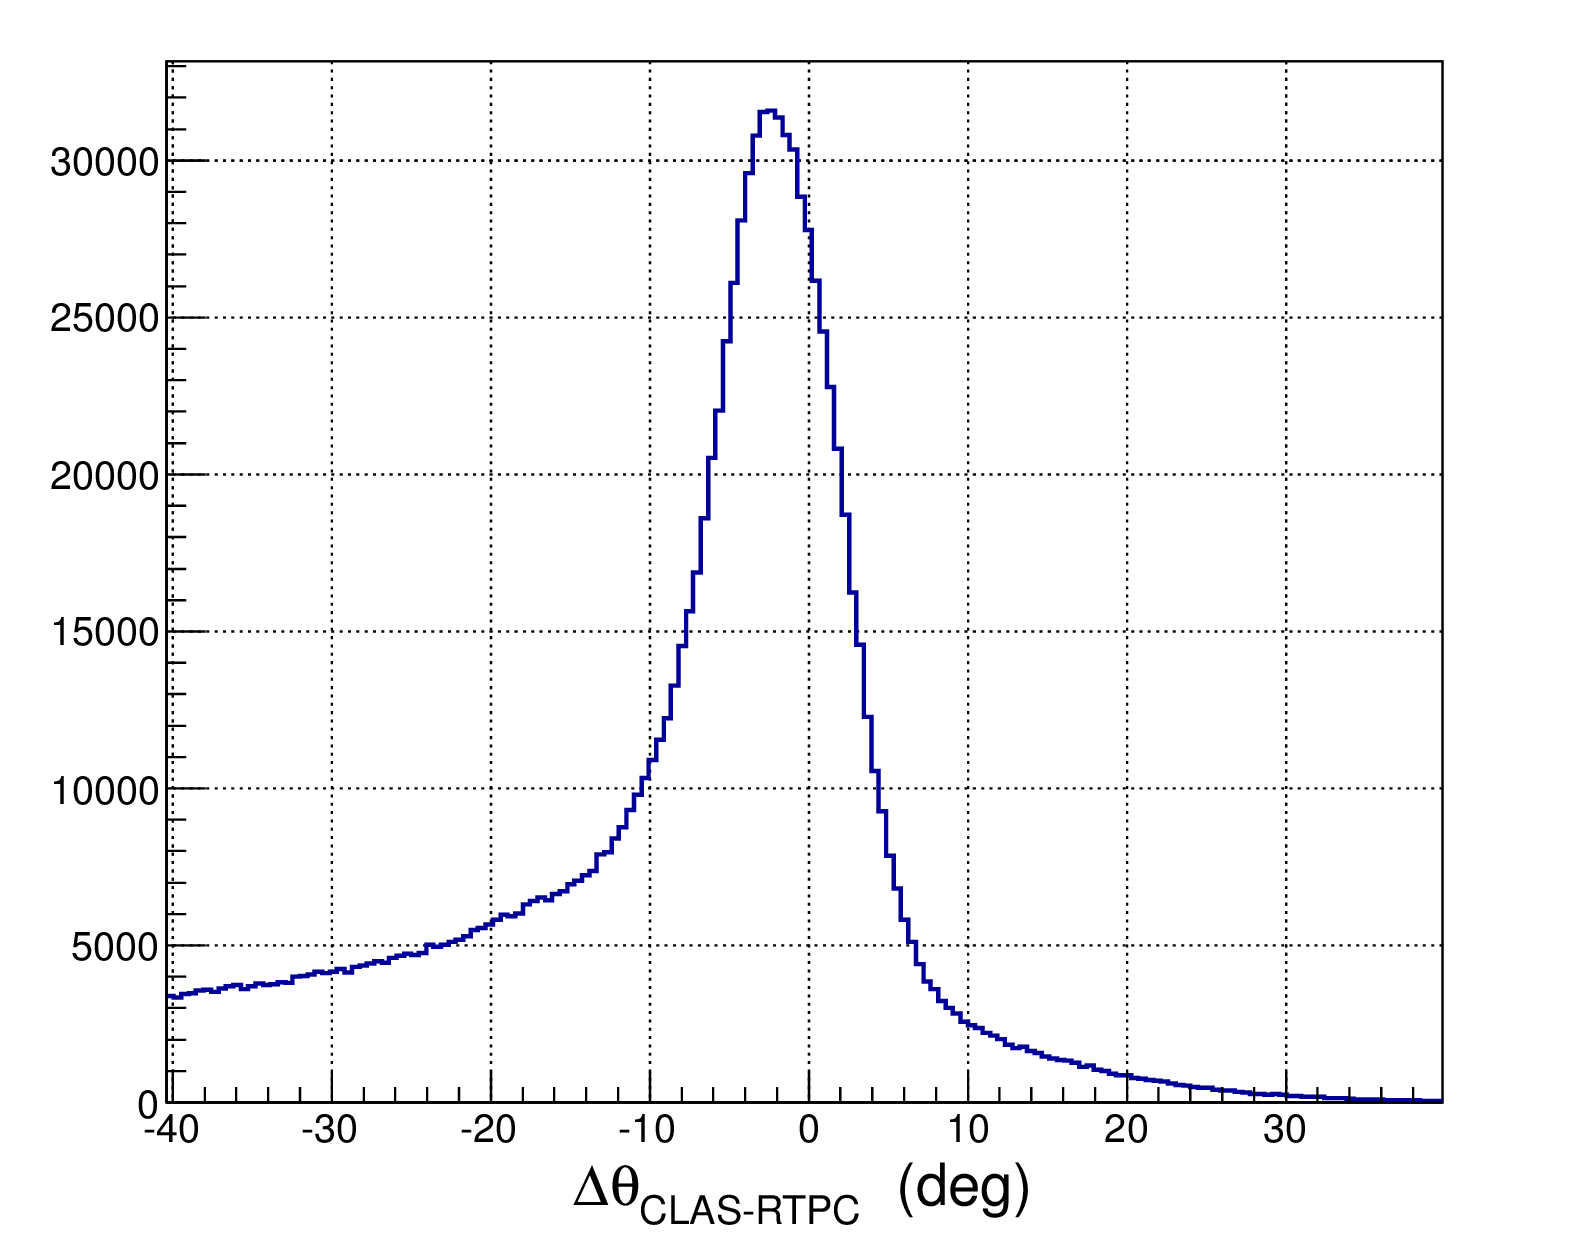
\includegraphics[width=5.4cm]{dtheQ.png}
    \caption{\label{fig:elastics}The CLAS-RTPC differences used for elastic event selection: $\delta z$, $\delta \phi$, and $\delta \theta$, left to right.  Each plot has a cut on the other two peaks.}%  Gaussian sigmas are roughly 8mm, 3deg and 4deg, respectively.}
\end{figure}
\begin{figure}[htbp]\centering
    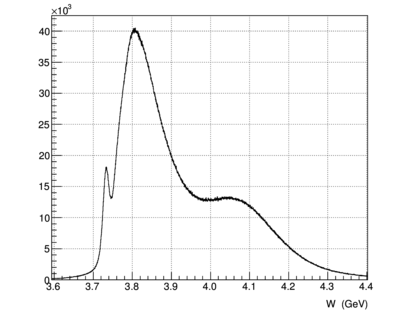
\includegraphics[width=7cm,height=5.3cm]{Wall_small.png}
    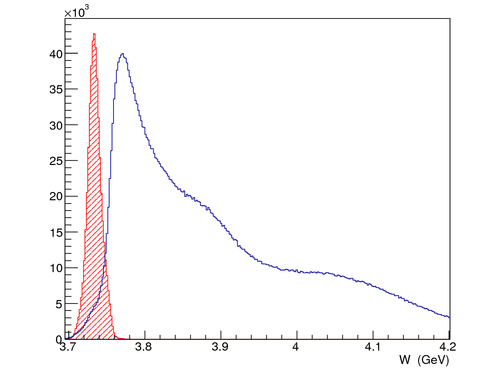
\includegraphics[width=7cm]{W_small.png}
    \caption{\label{fig:elasticsW}The W distribution for all events with one good electron (left).   The right panel adds the requirement of one good RTPC track matching the $z$-vertex of the electron, for events passing (red) and failing (blue) $\Delta\theta$ and $\Delta\phi$ cuts in Fig. \ref{fig:elastics}.}
\end{figure}

\subsection{RTPC Occupancy}
The occupancies of the 3200 RTPC channels are used to identify bad pads that should be discarded from reconstruction.
The raw occupancy for all RTPC pads in 1.206 GeV EG6 data is shown in the top panel Fig.\ref{fig:occ}.
After selecting elastic $^4$He tracks, the occupancy is shown in the lower panel of Fig.\ref{fig:occ}, where the combined acceptance of CLAS and the RTPC is visible.
Pads with occupancy below 1\% of the average are marked as bad and rejected in the reconstruction code and are accounted for in the path length calculation for $\frac{dE}{dx}$ in Section ~\ref{sec:measureddedx}.

The axis labels {\it column} and {\it row} notate the {\it pad}\# on the surface of the GEM and correspond to $z$ and $\phi$ directions, respectively.  The upstream end of the RTPC is at {\it column}=0, 10 cm from the center.  {\it Row}=0 corresponds to $\phi\sim -72^\circ$ and increases counter-clockwise looking downstream (there are $\sim36^\circ$ gaps at $\pm90^\circ$ due to support structure).  The two sections of the GEM are geometrically left/right symmetric and cover {\it rows} 0-39 and 40-79.  Readout boards cover 8 {\it columns} and 2 {\it rows}, hence the 8x2 bad regions.
%\begin{figure}[htbp]\centering
%    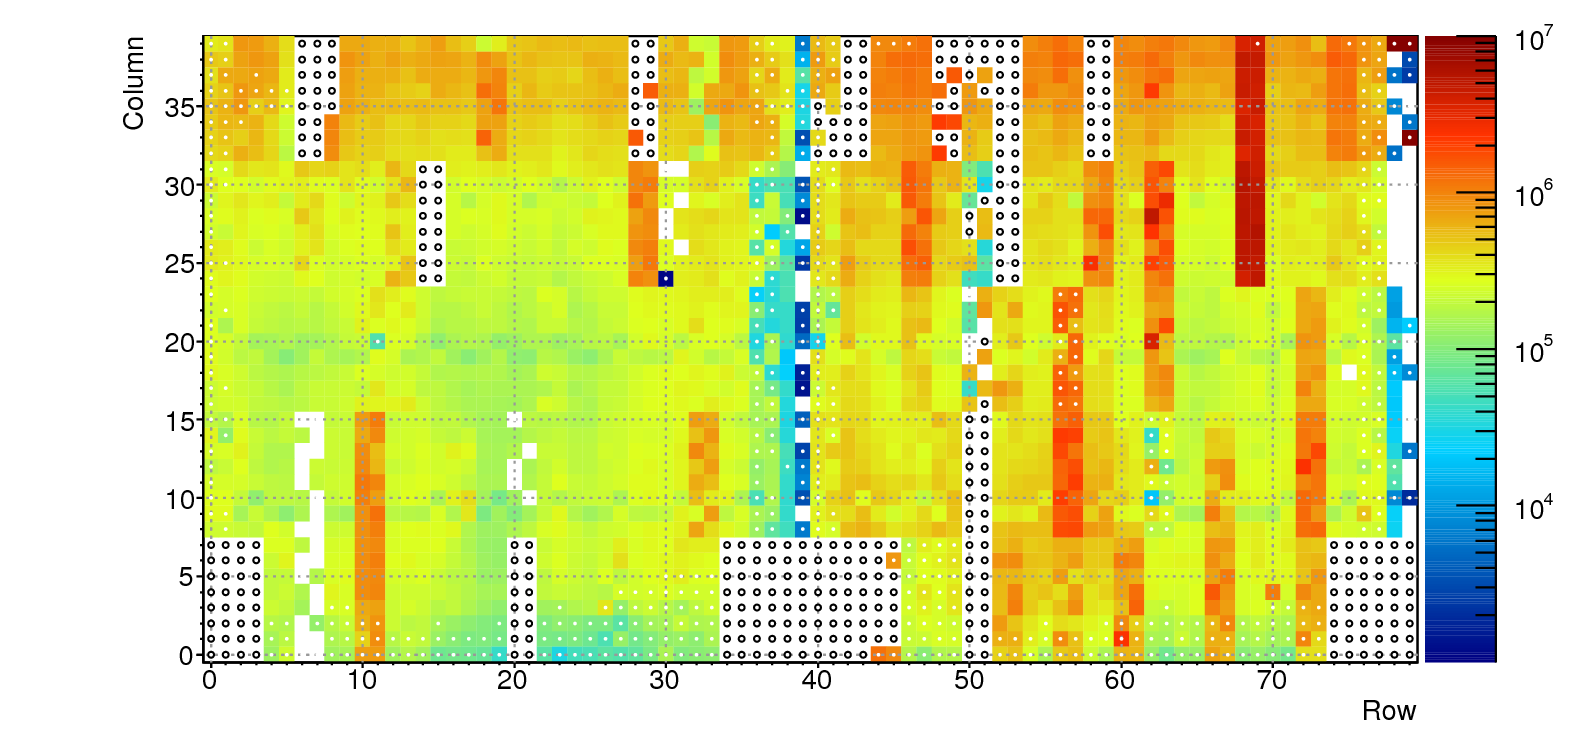
\includegraphics[width=17cm]{rawocc.png}
%    \caption{\label{fig:rawocc}The raw occupancy in the RTPC for all 1.206 GeV $^4$He runs.  Black dots denote pads that were already marked bad by previous studies.}
%\end{figure}
\begin{figure}[htbp]\centering
    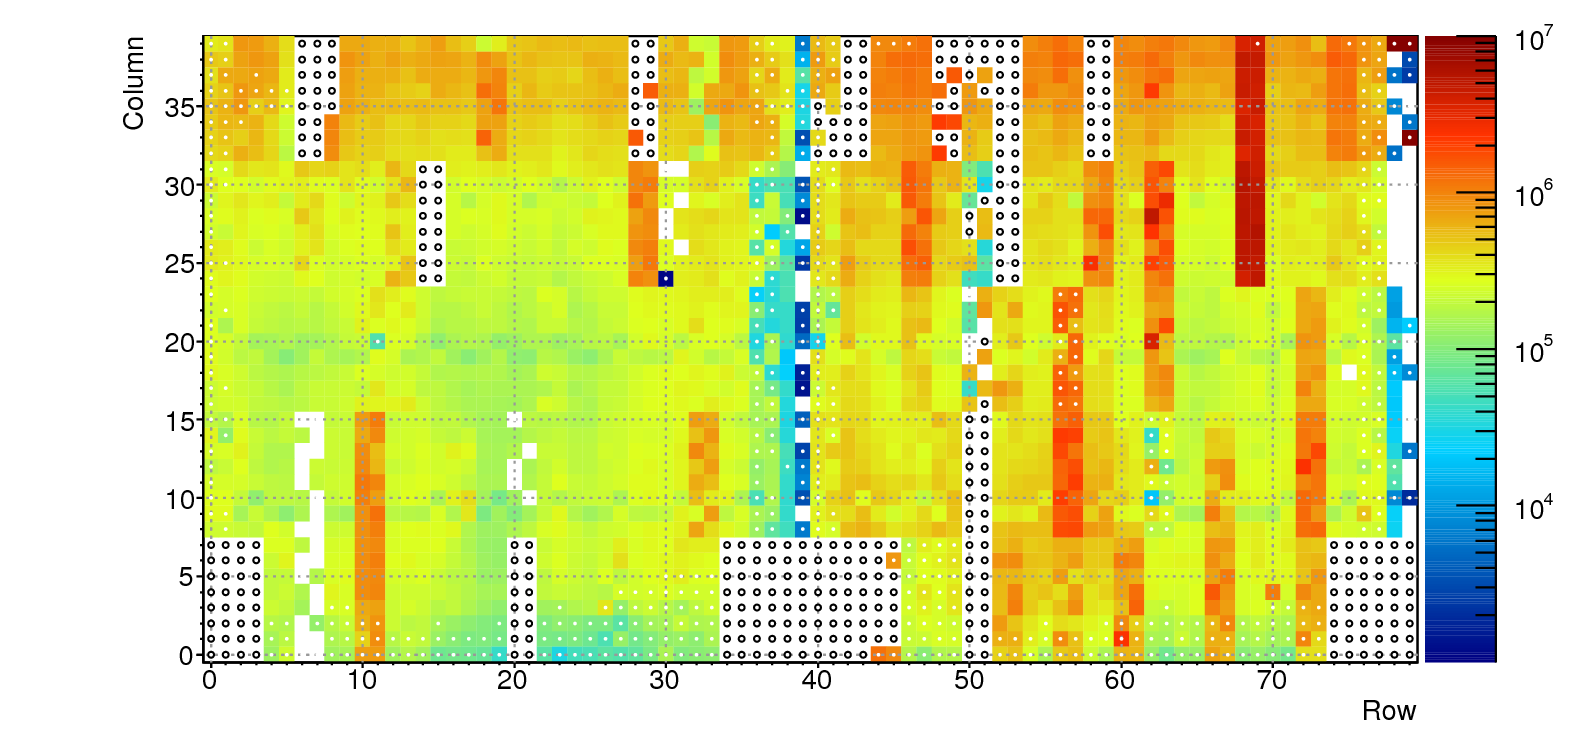
\includegraphics[width=11cm]{rawocc.png}
    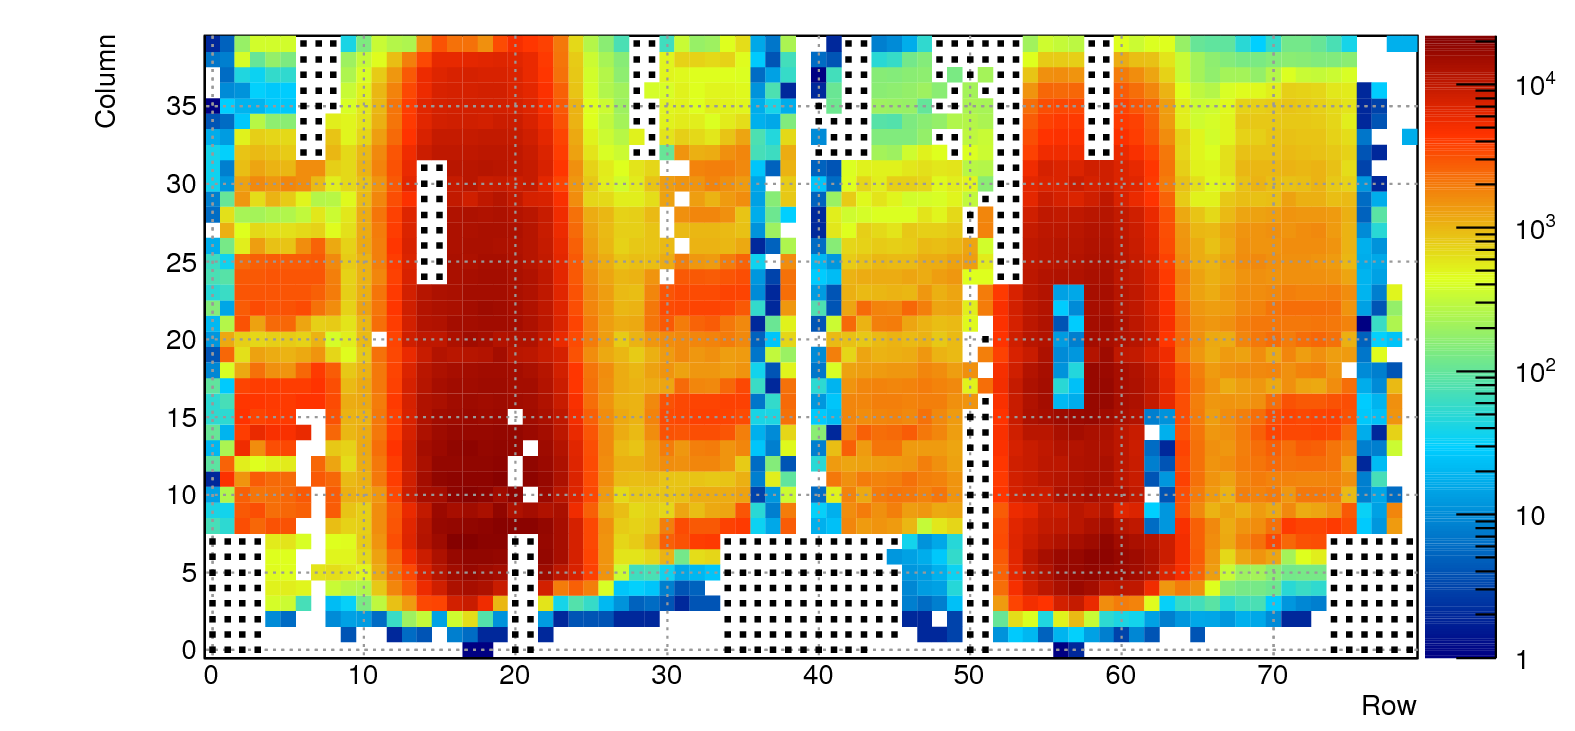
\includegraphics[width=11cm]{c1_b61482.png}
    \caption{\label{fig:occ}The raw occupancy (upper panel) of the GEM pads for all 1.206 GeV $^4$He runs, and the occupancy for elastic $^4$He tracks (lower panel) used for calibration.  Black dots denote pads there were already marked bad by previous studies.}
\end{figure}
%\begin{figure}[htbp]\begin{center}
%    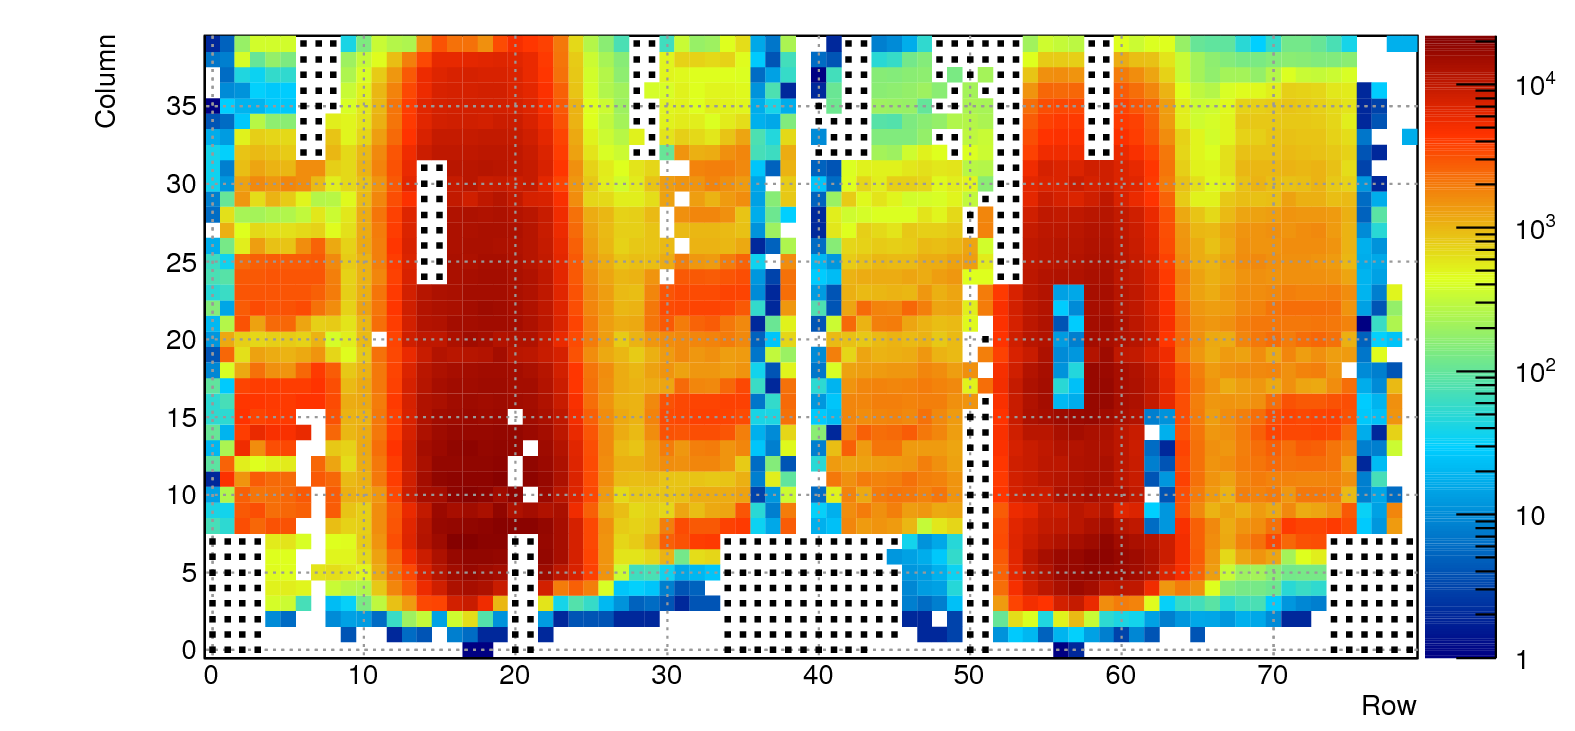
\includegraphics[width=17cm]{c1_b61482.png}
%    \caption{\label{fig:elaocc}The occupancy in the RTPC for all 1.206 GeV elastic $^4$He tracks for calibration.  Black dots denote pads there were marked bad by previous studies independent of elastic event selection.}
%\end{center}
%\end{figure}
\subsection{Calibration Method}
The gains of each pad are determined by calculating the average of the ratio of the measured and expected $\frac{dE}{dx}$, similar to the method used by BoNuS \cite{bonusgains}.  To do this, two histograms with 3200 bins corresponding to the 3200 channels are created. For every elastic $^4$He track, in one histogram the contents of the bin corresponding to each hit pad is incremented by 1 for each of that pad's hits (the occupancy).  In the other histogram, the same is done but with an increment of $\frac{dE}{dx}^{\textrm{Measured}}/\frac{dE}{dx}^{\textrm{Expected}}$.
Dividing the ratio-weighted histogram by the occupancy results in the calibrated gain factors.

However, this is inherently iterative because $\frac{dE}{dx}$ is calculated for the full track length, which includes multiple pads.  The gains are observed to converge after a few iterations for the majority of the pads (top panel of Fig. \ref{fig:gains5pass}).  Near the edges of the acceptance the convergence is not as good.
\begin{figure}[htbp]\centering
    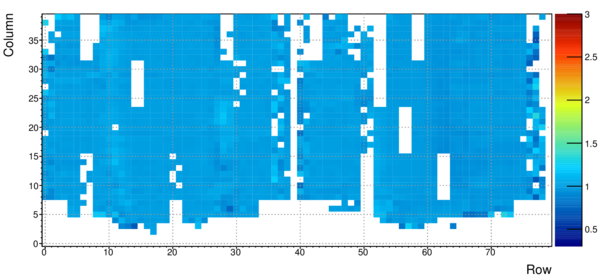
\includegraphics[width=11cm]{Gainrel_p56_v11_small.png}
    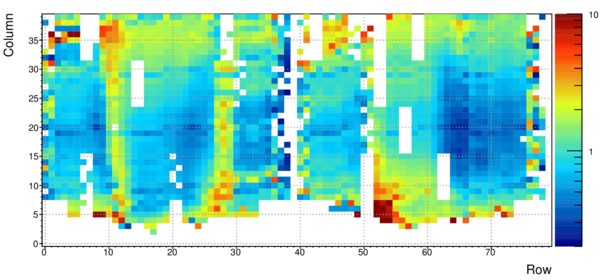
\includegraphics[width=11cm]{Gainabs_p6_v11_small.png}
    %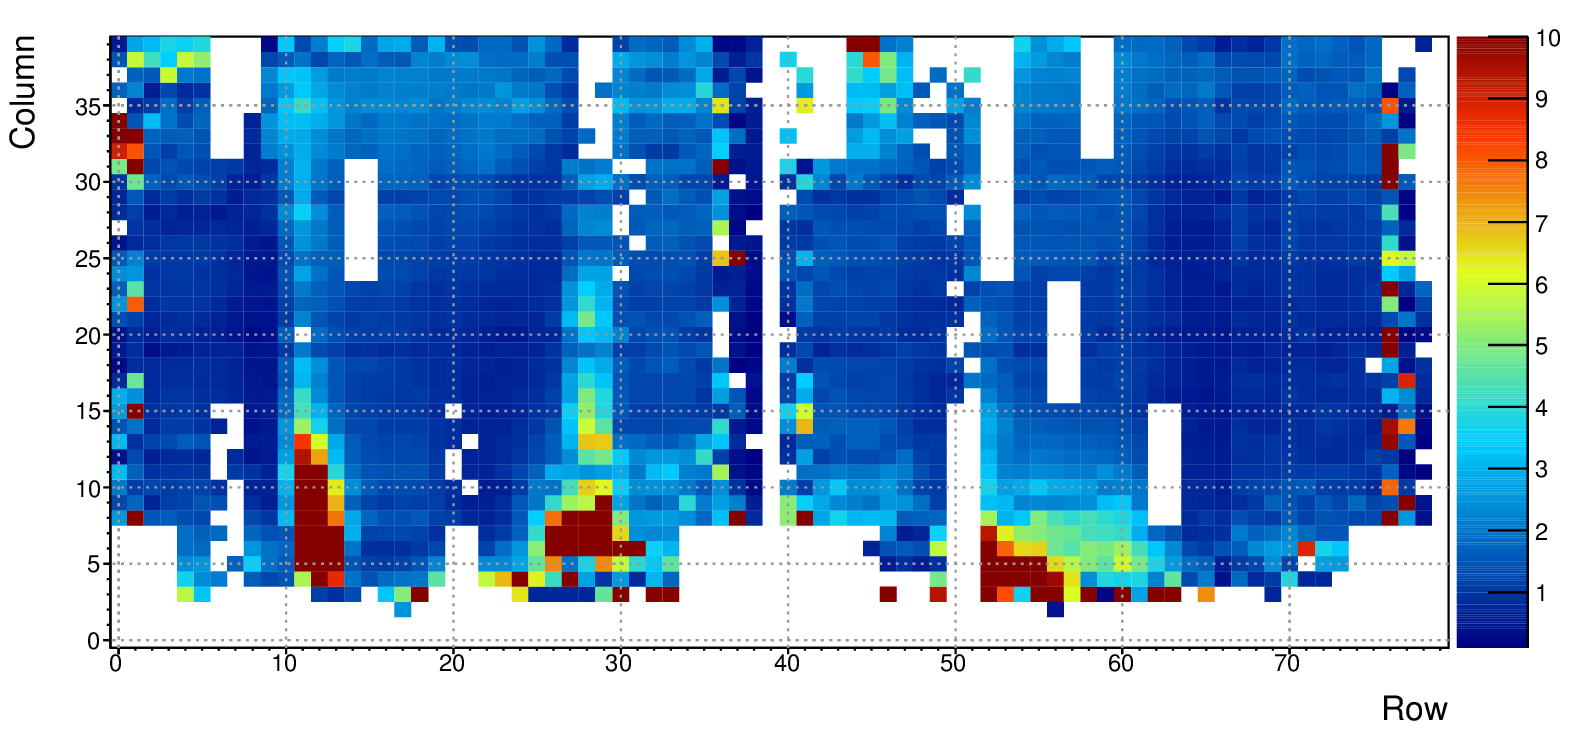
\includegraphics[width=14cm]{gainsabs_001-005.png}
    \caption{The relative change in the gains on the fifth iteration (top panel), and the final absolute gains (bottom panel).\label{fig:gains5pass}}
\end{figure}
%\begin{figure}[htbp]\centering
%    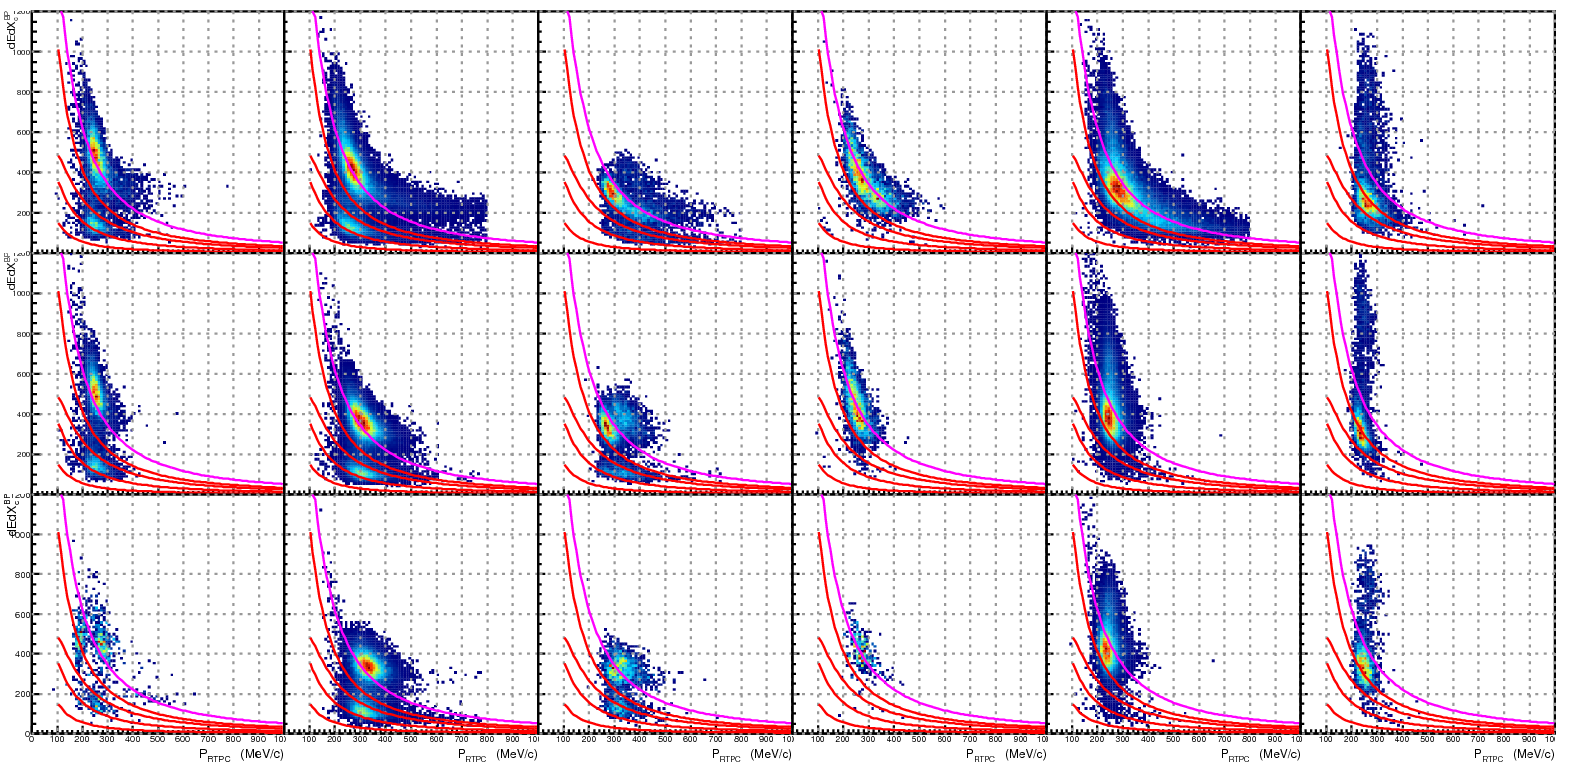
\includegraphics[width=17cm]{iter005__sectorsZCBP.png}
%    \caption{The $\frac{dE}{dx}$ versus momentum distribution for the six sectors (rows) and three $z$-vertex regions.\label{fig:dedx5pass}}
%\end{figure}

%and the resulting $\frac{dE}{dx}$ distribution versus momentum is shown in Fig. \ref{fig:dedx5pass}.

For a fine tuning, pads whose gains have not converged are reset to one and a $\frac{dE}{dx}$ cut around the expected $^4$He curve $\pm$1.5 times the distance to the $^3$He curve is applied to only calibrate using tracks in that range.  The final gain factors are shown in the bottom panel of Fig. \ref{fig:gains5pass}.  In order to keep the average gain near unity, the expected ``Bethe'' distribution was scaled by an overall normalization of 1333.

\section{Results}
The result is shown in Figs. \ref{fig:dedx5pass2} and \ref{fig:dedx5pass2_all} for $\frac{dE}{dx}$ versus momentum.
This analysis was done on 1.206 GeV {\it epass1v11} data, which was cooked with our best estimate of RTPC alignment and drift paths calibration \cite{rtpcalign,driftpaths}.  Those calibrations and the resulting gain calibrations shown here are included in {\it pass1v1}.


\begin{figure}[htbp]\centering
    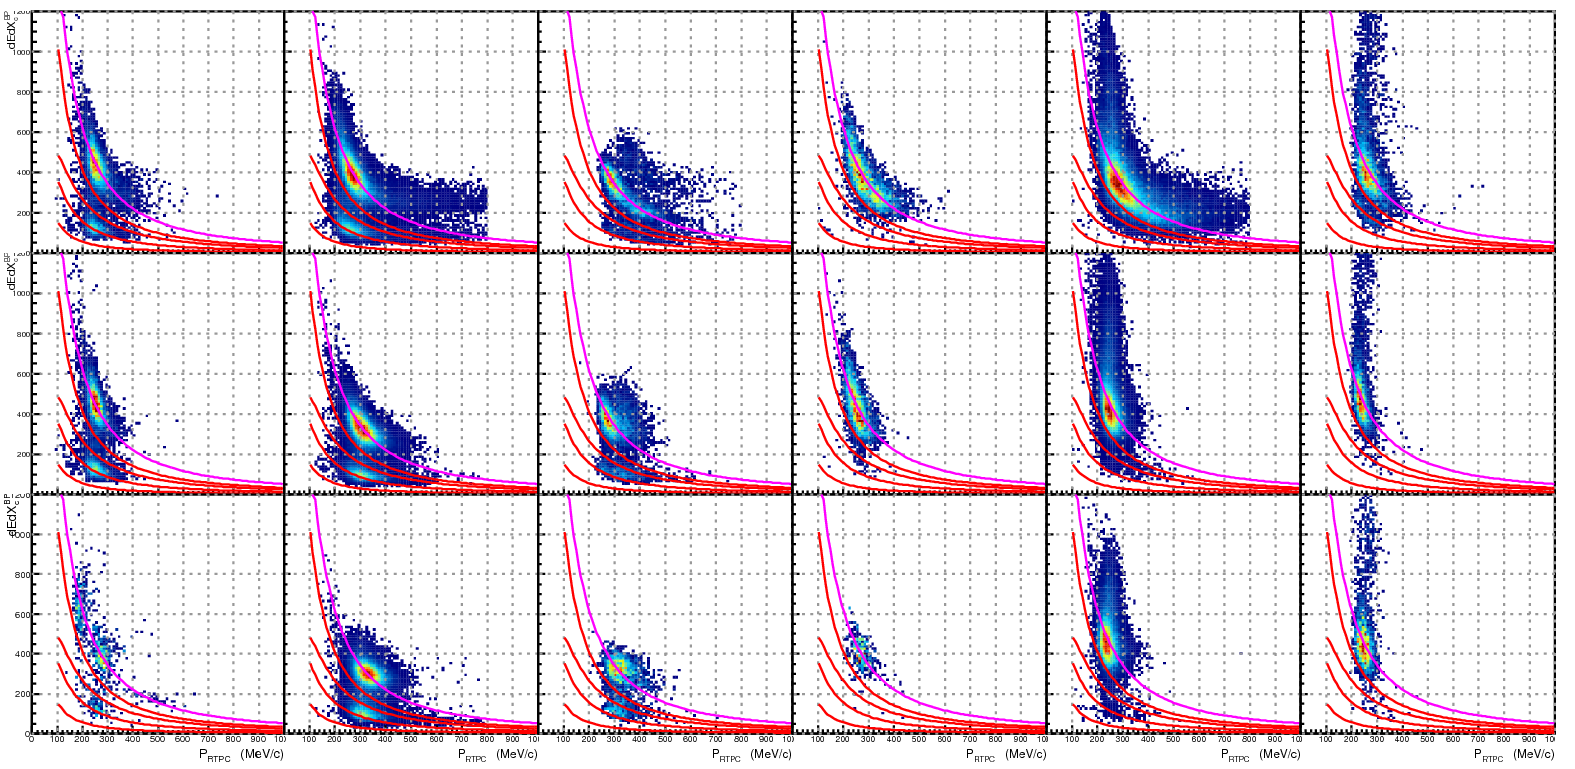
\includegraphics[width=17cm]{iter005__sectorsZCBPchopgainsrestartdedxcut.png}
    \caption{The RTPC's $\frac{dE}{dx}$ versus momentum distribution for tracks identified as elastic $^4$He.  The six columns correspond to the six CLAS sectors, and the three rows are $z$-vertex regions along the 20 cm RTPC.\label{fig:dedx5pass2}}
\end{figure}

\begin{figure}[htbp]\centering
    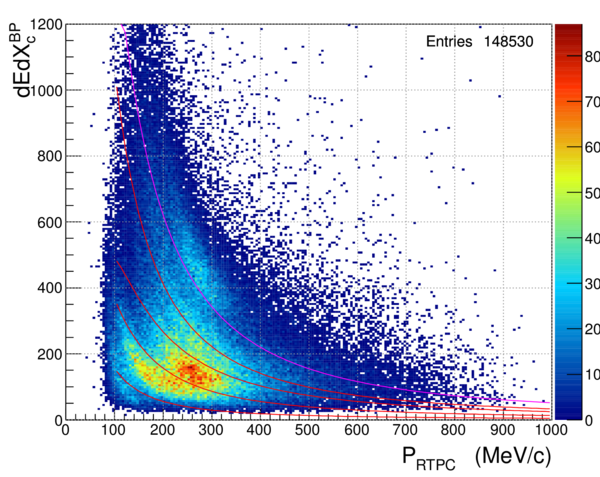
\includegraphics[width=10cm]{Left_dedxp_small.png}
    \caption{The RTPC's $\frac{dE}{dx}$ versus momentum distribution for all tracks with a matching electron $z$-vertex, integrated over the entire acceptance of the RTPC.  The $x$-axis is actually twice the measured momentum ($2\times p/q$), such that He isotopes are plotted with their true momentum, while H isotopes are plotted with twice their true momentum. \label{fig:dedx5pass2_all}}
\end{figure}

\newpage
\appendix{}
\section{Reconstructed RTPC BOS Banks}
There are two banks included in the cooked EG6 data, both ntuple and BOS files, that have information from the RTPC.
The motivation for the two banks is that a good preliminary analysis can be performed using only the {\it RTPC} bank, but the extra information of the {\it GCPB} bank may be useful for a most detailed analysis. 
\subsection{{\it GCPB} Bank}
The first bank is called {\it GCPB}, and its format has not been changed from what BoNuS used.  It includes information about all reconstructed tracks which involve at least 4 GEM pads, including detailed parameters related to helix fit quality, as well as the total number of hits and pads involved in the entire event.  Only false ``tracks'' with completely unreasonable or unphysical fit results are excluded.  A small selection of its variables is shown in Table \ref{tab:gcpbbank}.  For the {\it GCPB} bank, the BOS bank variable names are identical to the corresponding \texttt{h10} ntuple variable names.
\begin{table}[thpb]
    \caption{\label{tab:gcpbbank}Selection of {\it GCPB} BOS Bank variables}
    \begin{tabular}{p{4cm}r}
    \toprule[1.5pt]
    \texttt{x2/F}          & $\chi^2/N$ from helix fit \\
    \texttt{sdist/F}       & distance from cathode to first charge (mm)\\
    \texttt{edist/F}       & distance from last charge to GEM (mm)\\
    \texttt{dca/F}         & beamline DOCA (mm)\\
    \texttt{vtl/F}         & path length in drift region (mm)\\
    \texttt{r\_o/F}        & radius of curvature (mm)\\
    \texttt{q\_tot/F}      & total charge in the track\\
    \texttt{tothits/F}     & total number of GEM hits in the event\\
    \texttt{npd\_track/F}  & total number of pads in the track\\
    \texttt{npd\_event/F}  & total number of pads in the event\\
    \bottomrule[1.5pt]
\end{tabular}
\end{table}
\subsection{{\it RTPC} Bank}\label{sec:rtpcbank}
The second bank is newly created for EG6 and called {\it RTPC}.  It includes only the best tracks (see Table \ref{tab:rtpccuts} for criteria) and copies of the high-level variables from {\it GCPB}, but with the addition of a badpad-corrected $\frac{dE}{dx}$ and energy-loss corrected vertex momentum, as well as a pointer to the track in the {\it GCPB} bank.  The {\it RTPC} bank also includes a simple particle identification scheme based upon which of the five Bethe-Bloch curves ($^1$H,$^2$H,$^3$H,$^3$He,$^4$He) the measured $\frac{dE}{dx}$ is closest to:  \#1 is the best match, \#5 is the worst match.  The full variable list for the {\it RTPC} bank is shown in Table \ref{tab:rtpcbank}.  The numbering convention for pid is shown in Table \ref{tab:pidconvention}; the proton uses the PDG standard while the rest are GEANT3 values.  For the {\it RTPC} bank, the \texttt{h10} ntuple variable names are identical to their corresponding BOS bank variables, except prefixed by ``\texttt{rtpc\_}''.
\begin{table}[thpb]
    \caption{\label{tab:rtpccuts}Track Cuts for {\it RTPC} BOS Bank in EG6 {\it pass1v1}}
    \begin{tabular}{c}
    \toprule[1.5pt]
    -110 mm $<$ $z$-vertex $<$ +110 mm \\
    -5 mm $<$ edist $<$ +10 mm \\
    -5 mm  $<$ sdist $<$ +5 mm \\
    0.3   $<$ $\chi^2$ $<$  3 \\
    $N_{\textrm{pads}} > 3 $\\
    $r_0>0$ \\
    \bottomrule[1.5pt]
\end{tabular}
\end{table}
\begin{table}[thpb]
    \caption{\label{tab:rtpcbank}Complete {\it RTPC} BOS Bank Definition for EG6 {\it pass1v1}}
    \begin{tabular}{p{4cm}r}
    \toprule[1.5pt]
    \texttt{id1/I}        & pid for hypothesis \#1\\
    \texttt{id2/I}        &  pid for hypothesis \#2\\
    \texttt{id3/I}        &  pid for hypothesis \#3\\
    \texttt{id4/I}        &  pid for hypothesis \#4\\
    \texttt{id5/I}        &  pid for hypothesis \#5\\
    \texttt{p1/F}         &  vertex momentum for hypothesis \#1  (MeV)\\
    \texttt{p2/F}         &  vertex momentum for hypothesis \#2  (MeV)\\
    \texttt{p3/F}         &  vertex momentum for hypothesis \#3  (MeV)\\
    \texttt{p4/F}         &  vertex momentum for hypothesis \#4  (MeV)\\
    \texttt{p5/F}         &  vertex momentum for hypothesis \#5  (MeV)\\
    \texttt{poverq/F}     &  drift region momentum divided by charge (MeV)\\
    \texttt{dedx/F}       &  ADC/mm\\
    \texttt{dedx2/F}      &   ADC/mm with badpad correction\\
    \texttt{theta/F}      &   track polar angle at vertex (radians)\\
    \texttt{phi/F}        &   track azimuthal angle at vertex (radians)\\
    \texttt{vz/F}         &   $z$-vertex relative to RTPC-center (mm)\\
    \texttt{bad/F}        &   fraction of path length subtended by badpads\\
    \texttt{gcpb/I}       &   pointer to GCPB bank (c-style array index)\\
    \bottomrule[1.5pt]
\end{tabular}
\end{table}
\begin{table}[thpb]
    \caption{\label{tab:pidconvention}Numbering Convention for PID in the {\em RTPC} Bank}
    \begin{tabular}{p{2cm}r}
    \toprule[1.5pt]
    p & 2212 \\
    d & 45\\
    $^3$H & 46\\
    $^3$He & 49\\
    $^4$He & 47\\
    \bottomrule[1.5pt]
\end{tabular}
\end{table}

\clearpage
\newpage
\section{Further Studies}
Various corrections to the method were investigated.  So far, only the bad path length of Section \ref{sec:measureddedx} is found to be significant, but two others are documented here for posterity.
%The expected average instantaneous energy deposition is given directly by Eq. \ref{eq:bb}.  However, as the momentum decreases while the nuclei transverse the drift region, we are actually measuring an effective $\frac{dE}{dx}$ biased towards the latter half of the path length.  Additionally, some regions of the path length were not measured at all due to bad pads.  Corrections are applied to account for these effects.

\subsection{Pedestals}
The RTPC data acquisition used pedestals to subtract from the ADCs, however a study was done to determine if improvement is possible.
The trigger for data aquisition was at least 3 consecutive TDC tics with ADC values above a threshold of 35.
Then those three or more ``plateau'' hits and their 6 neighboring tics (3 on either side) are recorded in the TPC6 raw BOS bank.

The pedestals were reanalyzed by categorizing hits based upon their relationship to the plateau in the TPC6 bank: {\it on}, {\it off} and {\it far}, where the first two are obvious and {\it far} means more than two TDC tics from the plateau.  Using all plateaus found in the raw data, the ADC distribution for {\it far} hits are shown in Fig.\ref{fig:far} and confirm that the right half of the RTPC is much noisier.%, and suggestive that a further pedestal correction may be useful.

\begin{figure}[htbp]\centering
    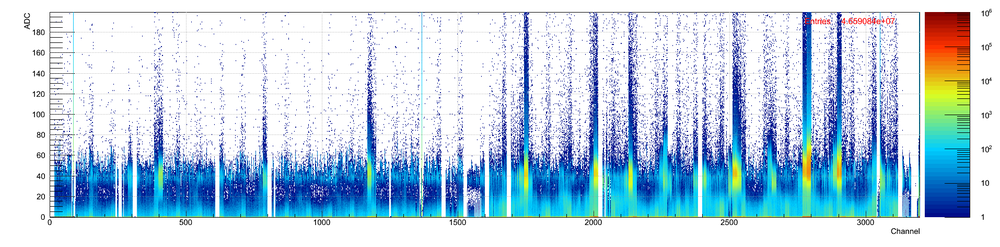
\includegraphics[width=17cm]{Rtpcadcs_far_small.png}
    \caption{The ADC distribution for the 3200 RTPC channels for only hits that are {\it far} from a plateau.\label{fig:far}}
\end{figure}

There is however, already a event-by-event noise cut in the reconstruction code that ignores pads that have more than 30 hits in a given event.  Applying this same cut, the ADC level of {\it far} hits is much reduced.  Trying an even tighter cut of 15 hits drops the {\it far} hits to almost zero for the large majority of pads (Fig.\ref{fig:relped}).  Based upon this, it is concluded that the {\it far} from plateau hits that are available in the raw data are likely not a stable estimate of the pedestal.

\begin{figure}[htbp]\centering
    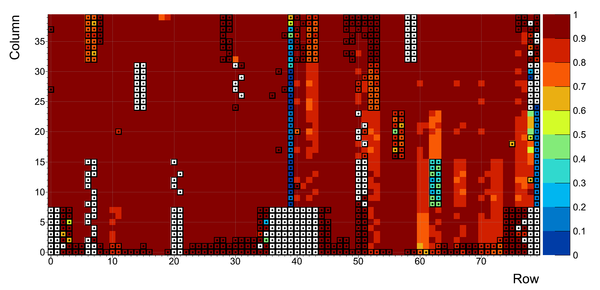
\includegraphics[width=11cm]{Eg6rtpc_pedestal_NEW15_small.png}
    \caption{The average relative difference between ADC values for {\it on} and {\it far} hits (see text) for when the pads have less than 15 hits per event.  The $z$-axis is $\frac{N_{on}-N_{far}}{N_{on}}$.\label{fig:relped}}
\end{figure}

Nevertheless, attempt was made to see if any improvement could be had by applying pedestals derived from the {\it far} hits.  While the number of reconstructed tracks did increase by a few-\%, the measured $\frac{dE}{dx}$ vs momentum distributions were largely unaffected after recalibration with new pedestals, and the number of elastic tracks reconstructed was unaffected.  A likely reason lies in the facts that geometric outliers were already rejected upon second iteration of the helix fit, and hits are weighted by their charge in the fit.  One interpertation is that the hits' ADCs that were largely reduced by this new pedestal, or rejected by it, were not contributing significantly anyway.

\subsection{Energy Loss Bias}
As the nucleus travels through the drift region it of course loses energy, as this is the basis of the RTPC.  But this means its $\frac{dE}{dx}$ increases along its path length.  The total measured energy deposition should then be biased towards the latter part of the trajectory in the drift region.  A calculation was done to estimate this effect, shown in Fig. \ref{fig:bias}, with the result that at the elastic kinematics used for calibration ($\sim$300 MeV/c and track length close to 3 cm), the effect is negligible.  At the most extreme kinematics measureable by the RTPC (small polar angle and low momentum), the effect is below 5\%.  Therefore, up to now this has been ignored as a high order effect.
\begin{figure}[htbp]\centering
    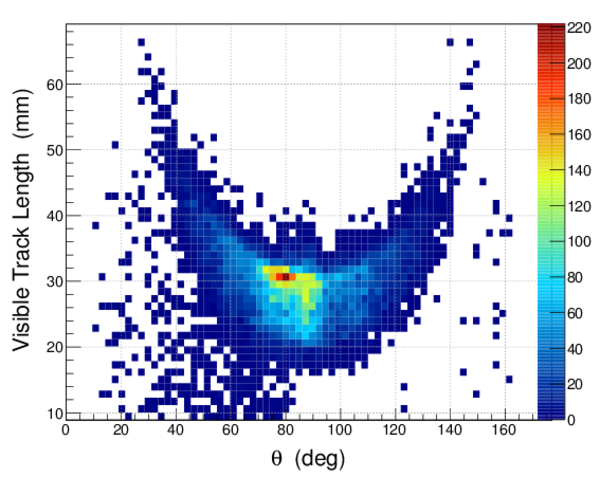
\includegraphics[width=8cm]{Vtl_theta_1gev.png}
    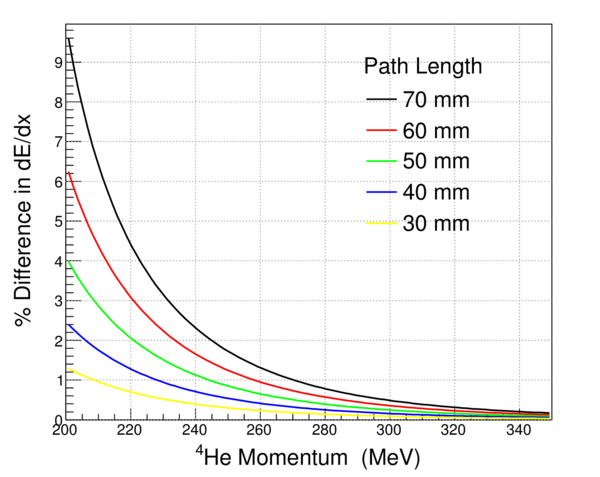
\includegraphics[width=8cm]{Biasbb_alpha.png}
    \caption{On left is the distribution of tracks measured in the RTPC;  the path length in the drift region is shown as a function of track polar angle.  On right is the expected relative difference between the average $\frac{dE}{dx}$ and that at the midpoint of the drift region.\label{fig:bias}}
\end{figure}
%\subsection{Truncated $\frac{dE}{dx}$}


\bibliography{tpcgaincal}
\end{document}

